\section{Fundamental Algorithms and Auxiliary Definitions}\label{sec:auxdefs}
In this section, we present the fundamental algorithms and auxiliary definitions used in our formalization.
Some of them are auxiliary functions, others are however important ones as they
directly implement our algorithm for method lookup.
%\bruno{I felt like there's not enough explanation/context in this
 % section. It is just dumping definitions without connecting them and
 % their purpose properly.}
 
\bruno{used for what and where?}\haoyuan{todo: used for where}

\subsection{Method Lookup Algorithm in \mbody{}}
Before showing the definition of \mbody{}, we start with several examples of method lookup, as shown in Figure~\ref{fig:examplesmbody}. Note that we use \lstinline|m| to denote an original method, and ``\lstinline|m|$\uparrow$\lstinline|A|'' for hierarchical overriding on \lstinline|A|. For each small example, the result gives the interface to which $m$ is dispatched. (a) is our old friend example for unintentional method conflicts (triangle inheritance); (b) and (c) demonstrate
that hierarchical dispatch can find the most specific original method and hierarchical overriding method. More interesting are the two bad examples (d) and (e), they both fail on $\mbody$. (d) is the well-known diamond inheritance, where $\mbody(m, D, A)$ is \Undefined; (e) is again a diamond conflict because the two hierarchical overriding methods are overriding the same branch. Both counter-examples imply that \lstinline|(A)new D().m()| will
lead to ambiguity, and in order to ensure type soundness, both of them have to be rejected by the type checker. Our model guarantees this by the interface checking rule\textsc{(T-Intf)} in Figure~\ref{fig:typingrules}. \haoyuan{need better explanation on these examples.}

Now we present the formal definition of \mbody{} that gives the expected results of the above mentioned examples. 

\begin{flalign*}
	& \rhd \textit{Definition of } \mbody(m, I_d, I_s): & \\
	& \bullet \mbody(m, I_d, I_s) = (J, \overline{I_x} \; \overline{x}, I_e \; e_0) & \\
	& \indent\indent \textrm{with: } \mostSpecific(m, I_d, I_s) = \{I\} & \\
	& \hspace{.77in} \mostSpecificOverride(m, I_d, I) = \{J\} & \\
	& \hspace{.77in} J[m\ \kwoverride\ I] = \method{I_e}{m}{I_x}{x}{I}{e_0} & \\
	& \bullet \mbody(m, I_d, I_s) = (J, \overline{I_x} \; \overline{x}, I_e \; \o) & \\
	& \indent\indent \textrm{with: } \mostSpecific(m, I_d, I_s) = \{I\} & \\
	& \hspace{.77in} \mostSpecificOverride(m, I_d, I) = \{J\} & \\
	& \hspace{.77in} J[m\ \kwoverride\ I] = \absmethod{I_e}{m}{I_x}{x}{I} & \\
\end{flalign*}
$\mbody(m, I_d, I_s)$ denotes the method body lookup function.
We use $I_d, I_s$, since $\mbody$ is usually invoked by a receiver of a method $m$, with its dynamic type $I_d$ and static type $I_s$. Such a function returns the most specific method implementation, more
accurately, its parameters, returned expression (empty for abstract methods) and the types. It considers both originally-defined methods and hierarchical overriding methods, so $\mostSpecific$ and $\mostSpecificOverride$ (see the definition in Section~\ref{sec:mostSpecific} and Section~\ref{sec:mostSpecificOverride}) are both invoked.

To calculate $\mbody(m, I_d, I_s)$, the invocation of $\mostSpecific$ looks for the most specific original methods and their interfaces, and expects a singleton set, so as to avoid unambiguity. Furthermore, the invocation of $\mostSpecificOverride$ also expects a unique (unambiguous) most specific hierarchical override. And finally the target method is returned.

\haoyuan{Need more examples?}\bruno{ask Marco.}
\begin{figure*}[t]
	\centering
	\vspace{-1ex}
	\begin{tabular}{ccc}
		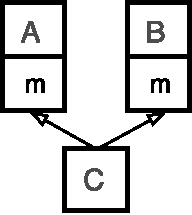
\includegraphics[width=1.5cm]{pics/P1.pdf}\hspace{4pt} &
		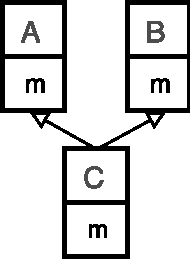
\includegraphics[width=1.5cm]{pics/P2.pdf}\hspace{4pt} &
		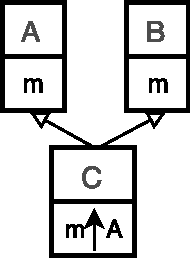
\includegraphics[width=1.5cm]{pics/P3.pdf}\hspace{4pt} \\
		(a) $\mbody(m,C,A) = (A,...)$\ \ \  & (b) $\mbody(m,C,A) = (C,...)$\ \ \  & (c) $\mbody(m,C,A) = (C,...)$
	\end{tabular} \\
	\begin{tabular}{cc}
		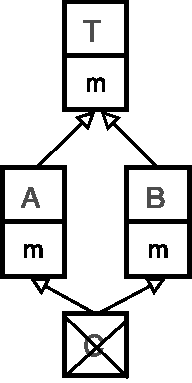
\includegraphics[height=3cm]{pics/P4.pdf}\hspace{4pt} &
		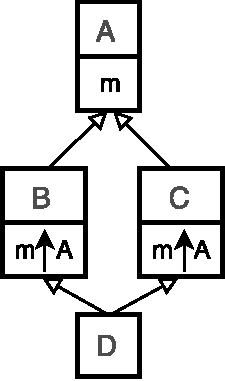
\includegraphics[height=3cm]{pics/P5.pdf}\hspace{4pt} \\ 
		(d) $\mbody(m,D,A) = \keyword{undefined}$\ \ \  & (e) $\mbody(m,D,A) = \keyword{undefined}$
	\end{tabular}
	\caption{Examples on $\mbody$. ``$\uparrow$'' stands for hierarchical overriding.}\label{fig:examplesmbody}
	%\saveSpaceFig
\end{figure*}


\subsection{Finding the Most Specific Origin: \mostSpecific}\label{sec:mostSpecific}
We proceed to give the definition of two core functions that support method lookup, namely \mostSpecific{} and \mostSpecificOverride. Generally,
$\mostSpecific(m, I, J)$ finds the set of most specific interfaces where $m$ is originally defined, they should be above $I$ and
along path $J$. ``Along path $J$'' means one should be either a subtype or a super type of $J$. Finally with $\prune$ (defined in Section~\ref{sec:otherdefs})
the overridden interfaces will be filtered out.

\begin{flalign*}
	& \rhd \textit{Definition of } \mostSpecific(m, I, J): & \\
	& \bullet \mostSpecific(m, I, J) = \prune(origins) & \\
	& \indent\indent \textrm{with: } origins = \{K \mid \subt{I}{K}, \textrm{ and } \subt{K}{J} \; \lor \; \subt{J}{K}, &\\
	& \hspace{1.62in} \textrm{ and } K[m\ \kwoverride\ K] \textrm{ is defined} \} &
\end{flalign*}
By the definition, an interface belongs to $\mostSpecific(m, I, J)$ if and only if:
\begin{itemize}
	\item It originally defines $m$;
	\item It is a super type of $I$;
	\item It is either a super type or a subtype of $J$ (including $J$ itself);
	\item Any subtype of it does not belong to the same result set because of $\prune$.
\end{itemize}

\subsection{Finding the Most Specifc Overriding: \mostSpecificOverride}\label{sec:mostSpecificOverride}
The $\mostSpecific$ function only focuses on original method implementations, all the hierarchical overriding methods are omitted during that step. On the other hand, $\mostSpecificOverride(m, I, J)$ has the assumption that $J$ defines an original $m$, and this function tries to find the interfaces with most specific implementations that hierarchically overrides such an $m$. Formally,

\begin{flalign*}
	& \rhd \textit{Definition of } \mostSpecificOverride(m, I, J): & \\
	& \bullet \mostSpecificOverride(m, I, J) = \prune(overrides) & \\
	& \indent\indent \textrm{with: } overrides = \{K \mid \subt{I}{K}, \; \subt{K}{J} \textrm{ and } K[m\ \kwoverride\ J] \textrm{ is defined} &
\end{flalign*}
By the definition, an interface belongs to $\mostSpecific(m, I, J)$ if and only if:
\begin{itemize}
	\item It is between $I$ and $J$;
	\item It hierarchically overrides $J.m$;
	\item Any subtype of it does not belong to the same set.
\end{itemize}


\subsection{Others}\label{sec:otherdefs}
Below we give other minor definitions of the auxiliary functions that are used in previous sections.

%%%%============================ I[m override J] ================%%%%%%%%
\begin{flalign*}
	& \rhd \textit{Definition of } I[m\ \kwoverride\ J]: & \\
	& \bullet I[m\ \kwoverride\ J] = \method{I_e}{m}{I_x}{x}{J}{e_0} & \\
	& \indent\indent \textrm{with: }
	  \kwinterface \; I \; \kwextends \; \overline{I} \; \{ \method{I_e}{m}{I_x}{x}{J}{e_0} \ldots \} & \\
	& \bullet I[m\ \kwoverride\ J] = \absmethod{I_e}{m}{I_x}{x}{J} & \\
	& \indent\indent \textrm{with: }
	\kwinterface \; I \; \kwextends \; \overline{I} \; \{ \absmethod{I_e}{m}{I_x}{x}{J} \ldots \} & \\
\end{flalign*}
Here $I[m\ \kwoverride\ J]$ is basically a direct lookup for method $m$ in the body of $I$, where such a method
overrides $J$ (like static dispatch). The method can be either concrete or abstract, and the body of definition is returned. Notice that
by our syntax, $I[m\ \kwoverride\ I]$ is looking for the originally-defined method $m$ in $I$.
%%%%============================ I[m override J] end================%%%%%%%%

%%%%============================ prune(set) ================%%%%%%%%
\begin{flalign*}
	& \rhd \textit{Definition of } \prune(set): & \\
	& \bullet \prune(set) = \{I \in set \; | \; \nexists J \in set\setminus I, J <: I\} &
\end{flalign*}
The $\prune$ function takes a set of
types, and filters out those that have subtypes in the same set. In the returned set,
none of them has subtyping relation to one another, since all super types have been removed.
%%%%============================ prune(set) end ================%%%%%%%%

%%%%============================ canOverride ================%%%%%%%%
\begin{flalign*}
	& \rhd \textit{Definition of } \canOverride(m, I, J): & \\
	& \bullet \canOverride(m, I, J) = True & \\
	& \indent\indent \textrm{with: } I[m\ \kwoverride\ I] = I_e \; m(\overline{I_x} \; \overline{x}) \; \kwoverride \; I \ldots & \\
	& \hspace{.77in} J[m\ \kwoverride\ J] = I_e \; m(\overline{I_x} \; \overline{y}) \; \kwoverride \; J \ldots &
\end{flalign*}
$\canOverride$ just checks that two original $m$ in $I$ and $J$ have the same type.
%%%%============================ canOverride end ================%%%%%%%%

%%%%============================ canInstantiate ================%%%%%%%%
\begin{flalign*}
	& \rhd \textit{Definition of } \canInstantiate(I): & \\
	& \bullet \canInstantiate(I) = True & \\
	& \indent\indent \textrm{with: } \forall J \in \mostSpecific(m, I, I), \mostSpecificOverride(m, I, J) = \{K\}, & \\
	& \hspace{.77in} \textrm{ and } K[m\ \kwoverride\ J] = \method{I_e}{m}{I_x}{x}{J}{e_0} &
\end{flalign*}
$\canInstantiate(I)$ checks whether interface $I$ can be instantiated by the keyword $\kwnew$.
$\mostSpecific(m, I, I)$ represents the set of branches $I$ inherits on method $m$. $I$ can be instantiated
if and only if for every branch, the most specific implementation is unambiguous and non-abstract.
%%%%============================ canInstantiate end ================%%%%%%%%
